\section{Research scope and evidence hierarchy}\label{sec:scope}
The title describes the intended C/P/V multi-agent research framework. It does not imply that the strongest result in this paper was generated by a language model. The repository contains three related but non-interchangeable lines of work: (i) an offline role-based agent implementation and bounded local LLM feasibility run, (ii) retrospective statistical grouping and ranking on Microsoft GUIDE, and (iii) a controlled synthetic study of evidence-gated reconstruction. We report each with its actual data, model, and evaluation status. This distinction is essential because attributing the synthetic holdout improvement to the LLM roles would change the treatment under study.

The C agent proposes an alert relationship, the P agent scores an incident candidate, and the V agent checks the support for claims and citations. The original architectural specification uses C--P--V as role names and proposes a revision loop. The \emph{frozen synthetic predictor} actually executes initial correlation, then verification of cross-fragment tokens, then deterministic ranking: C/V/P. The role naming and execution order answer different questions. The former is a software decomposition; the latter is the measured prediction path. Figure~\ref{fig:scope} makes the separation explicit.

\begin{figure*}[t]\centering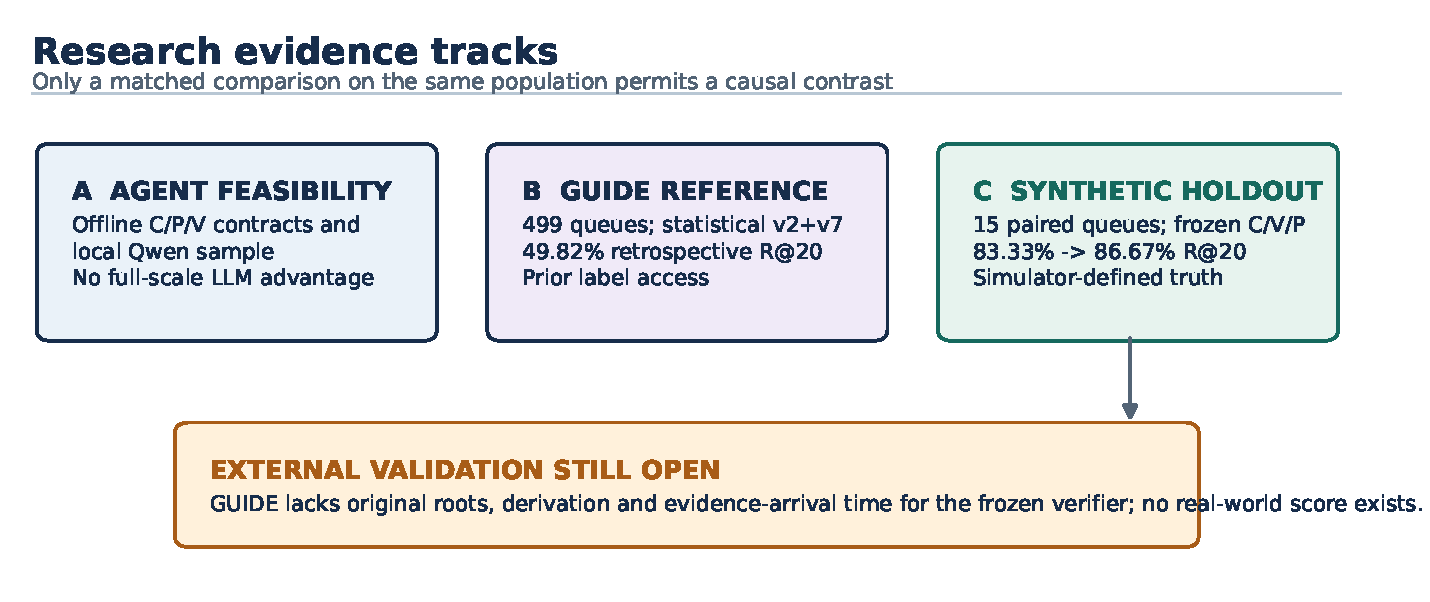
\includegraphics[width=.85\textwidth]{figures/study_tracks.pdf}
\caption{Three evidence tracks in the project. The local LLM and offline agent contracts demonstrate bounded execution; the retrospective GUIDE work evaluates a statistical reference on previously accessed labels; and the paired fresh synthetic holdout evaluates a deterministic evidence-gated method. Arrows identify conceptual inheritance, not a pooled training or performance cohort.}\label{fig:scope}\end{figure*}

\begin{table*}[t]\centering\footnotesize\caption{Claims permitted by the available evidence. ``Model'' refers to the actual measured predictor, rather than the project title.}\label{tab:scope}
\begin{tabularx}{\textwidth}{@{}p{.18\textwidth}p{.19\textwidth}p{.23\textwidth}Y@{}}\toprule
Track & Data and scope & Implemented method & Supported conclusion\\\midrule
Role contracts and local LLM & Synthetic fixtures; bounded 20-organization local prototype & C/P/V schemas, deterministic offline adapter; local Qwen prototype & Feasible orchestration and bounded model execution; no full-scale comparative LLM efficacy\\
Historical GUIDE & 499 organization queues; previously inspected labels & Entity-enabled candidates, v2 statistical pair grouping, v7 group ranker & Retrospective exploratory 49.82\% R@20 statistical reference, not a fresh confirmation\\
Controlled fresh holdout & 15 synthetic queues; 5,018 eligible alerts & Frozen deterministic initial correlator, evidence verifier, endpoint fallback and score & Paired synthetic 86.67\% versus 83.33\% R@20 under simulator truth\\
External readiness & GUIDE schema and field policy & Data and authorization audit; no frozen-verifier prediction & Real-world performance and shadow readiness unmeasured\\\bottomrule
\end{tabularx}\end{table*}

The fresh synthetic study is the paper's strongest \emph{confirmatory result within its generator family}. The retrospective GUIDE result provides context on realistic data volume and failure modes but cannot validate the synthetic provenance gate: GUIDE's available schema does not contain original observation roots, derivation ancestry, or receiver availability times. Neither set is used as the other's baseline. Distinct denominators, grouping semantics, and label access histories prohibit an aggregate performance number.

Our scientific questions are thus partitioned: can bounded roles and trace contracts represent an evidence-grounded SOC workflow; under what exact conditions can a verifier add a cross-fragment union; what changes in matched retrieval and safety when a narrow missing-process fallback is frozen; and what data must be acquired before an external test? The answers are an implemented architecture, a code-aligned decision rule, a paired controlled experiment, and an explicit negative readiness finding. The paper does not evaluate analyst productivity, incident response actions, deployed latency, or a head-to-head LLM versus non-LLM comparison.
